\def\baselinestretch{1}
\chapter{RESULTS} \label{chap:results}
    \minitoc
    \begin{center}
    	\emph{Abstract of chapter \ref{chap:results}}
    \end{center}
    
    \section{Source list}
    	The list of sources which were studied are listed in table \ref{tab:source-list} below.
    	
    	\renewcommand{\arraystretch}{1.5}
    	\begin{table}[!htb]
    		\centering
    		\caption{List of sources in dataset}
    		\label{tab:source-list}
			\begin{tabular}{cccccc}
			\hline
			\textbf{S. No.} & \textbf{Source} & \textbf{Type} & \textbf{Galaxy} & \textbf{\begin{tabular}[c]{@{}c@{}}R. A.\\ (degrees)\end{tabular}} & \textbf{\begin{tabular}[c]{@{}c@{}}Dec.\\ (degrees)\end{tabular}} \\ \hline
			{1} & {CAL 83} & {XRB} & {} & {85.89233} & {-68.37283} \\
			{2} & {RS Oph} & {SS} & {} & {267.55483} & {-6.70791} \\
			{3} & {RX J0019.8+2156} & {CV} & {MW} & {4.95802} & {21.94783} \\
			{4} & {RX J0527.8-6954} & {CV} & {} & {81.95345} & {-69.90247} \\
			{5} & {RX J0925.7-4758} & {XRB} & {MW} & {141.44167} & {-47.97148} \\
			{6} & {V3890 Sgr} & {CN} & {} & {277.68037} & {-24.01915} \\ \hline
			\end{tabular}
		\end{table}
		\renewcommand{\arraystretch}{2.2}
		
		\subsection{Supersoft X-ray count rates}
			\begin{landscape}
			\begin{table}[!htb]
				\centering
	    		\caption{SSS observation journal of dataset}
	    		\label{tab:sss-obs-list}
				\begin{tabular}{cccccccc}
				\hline
				\textbf{Source} & \textbf{Observatory} & \textbf{Instrument} & \textbf{\begin{tabular}[c]{@{}c@{}}Observation\\ (Obs. ID)\end{tabular}} & \textbf{\begin{tabular}[c]{@{}c@{}}Date\\ (yyyy-mm-dd)\end{tabular}} & \textbf{MJD} & \textbf{\begin{tabular}[c]{@{}c@{}}Exposure\\ (ks)\end{tabular}} & \textbf{\begin{tabular}[c]{@{}c@{}}Region\\ (keV)\end{tabular}} \\ \hline
				{CAL 83} & {XMM-Newton} & {EPIC-pn} & {0506531501} & {2008-08-12} & {54690.62} & {6.9} & {0.2--1.0} \\
				{RS Oph} & {XMM-Newton} & {EPIC-pn} & {0410180501} & {2006-10-09} & {54017.98} & {49.2} & {0.2--2.0} \\
				{RX J0019.8+2156} & {XMM-Newton} & {EPIC-pn} & {0047940101} & {2001-12-31} & {52274.77} & {58.1} & {0.2--0.5} \\
				{RX J0527.8-6954} & {XMM-Newton} & {EPIC-pn} & {0086770101} & {2000-12-19} & {51897.70} & {49.3} & {0.2--0.6} \\
				{RX J0925.7-4758} & {XMM-Newton} & {EPIC-pn} & {0111150101} & {2000-12-16} & {51894.46} & {61.1} & {0.3--1.0} \\
				{V3890 Sgr} & {XMM-Newton} & {EPIC-MOS1} & {0821560201} & {2019-09-14} & {58740.98} & {25.0} & {0.1--2.0} \\ \hline
				\end{tabular}
			\end{table}
			\end{landscape}
			
			The count rates of the sources as observed by the respective observatories in table \ref{tab:sss-obs-list} over the respective energy ranges are presented in the sub-figures in \ref{result:count-rate}.
			\begin{figure}[h!]
				\centering
				\caption{Count rates of individual sources in dataset in SSS regime}
				\label{result:count-rate}
				\subfloat[CAL 83 \label{count-rate:cal83}]{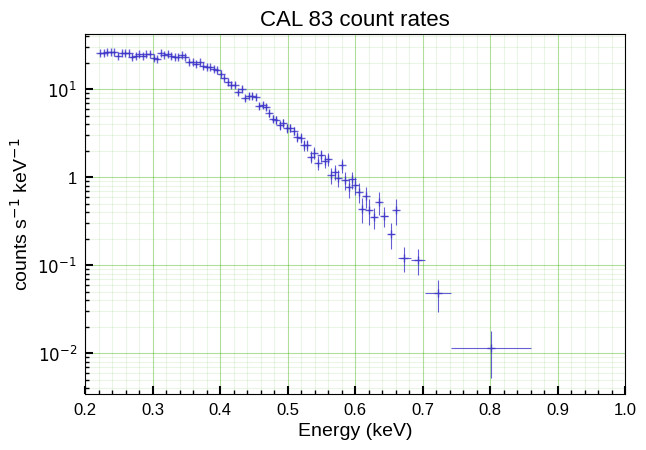
\includegraphics[width=0.45\textwidth]{counts/cal-83-pn_counts}} %\hfill
				\subfloat[RS Oph \label{count-rate:rsoph}]{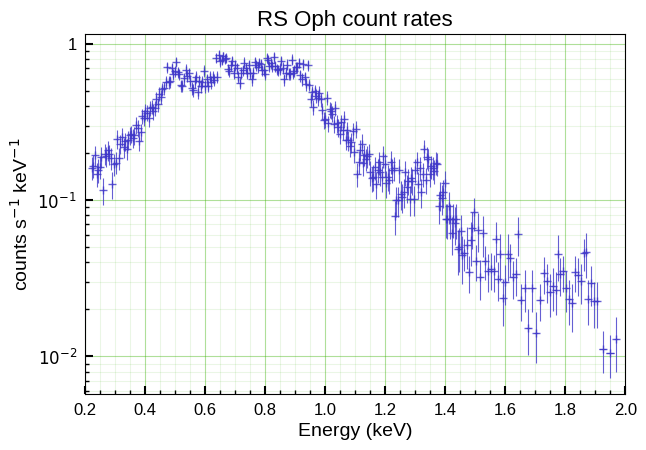
\includegraphics[width=0.45\textwidth]{counts/rs-oph-pn_counts}} %\hfill
				
				\subfloat[RX J0019.8+2156 \label{count-rate:rxj0019}]{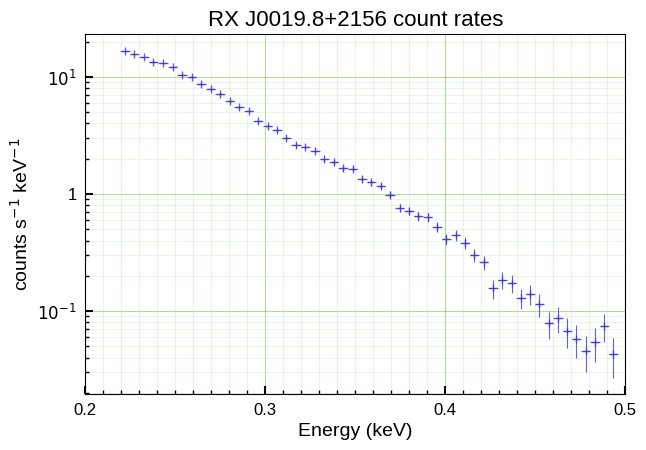
\includegraphics[width=0.45\textwidth]{counts/rx-j0019d8p2156-pn_counts}} %\hfill
				\subfloat[RX J0527.8-6954 \label{count-rate:rxj0527}]{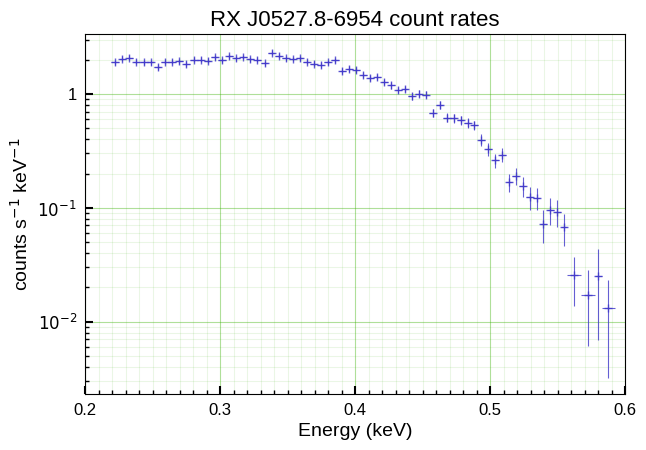
\includegraphics[width=0.45\textwidth]{counts/rx-j0527d8-6954-pn_counts}} %\hfill
				
				\subfloat[RX J0925.7-4758 \label{count-rate:mrvel}]{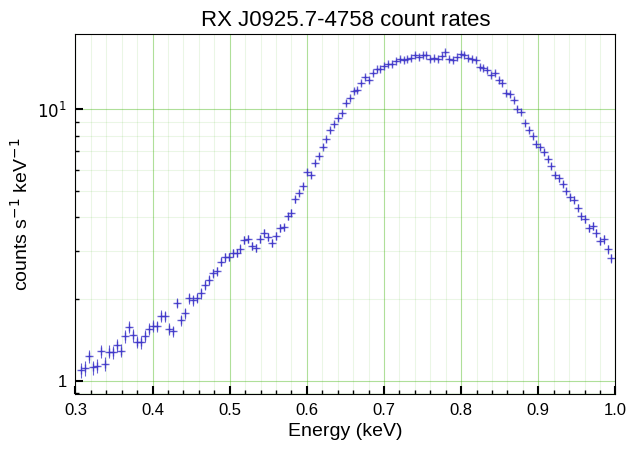
\includegraphics[width=0.45\textwidth]{counts/rx-j0925-4758-pn_counts}} %\hfill
				\subfloat[V3890 Sgr \label{count-rate:v3890}]{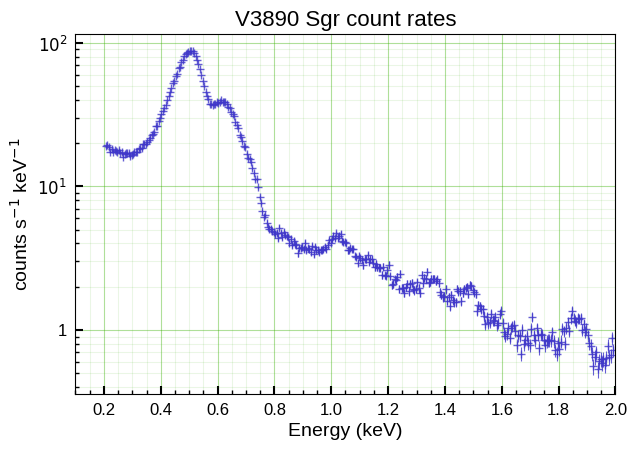
\includegraphics[width=0.45\textwidth]{counts/v3890-sgr-pn_counts}} %\hfill
			\end{figure}
			
			\begin{figure}[h!]
				\centering
				\caption{Count rates of all sources in dataset}
				\label{result:count-rate}
				\subfloat[Count rates of all sources \label{count-rate:cal83}]{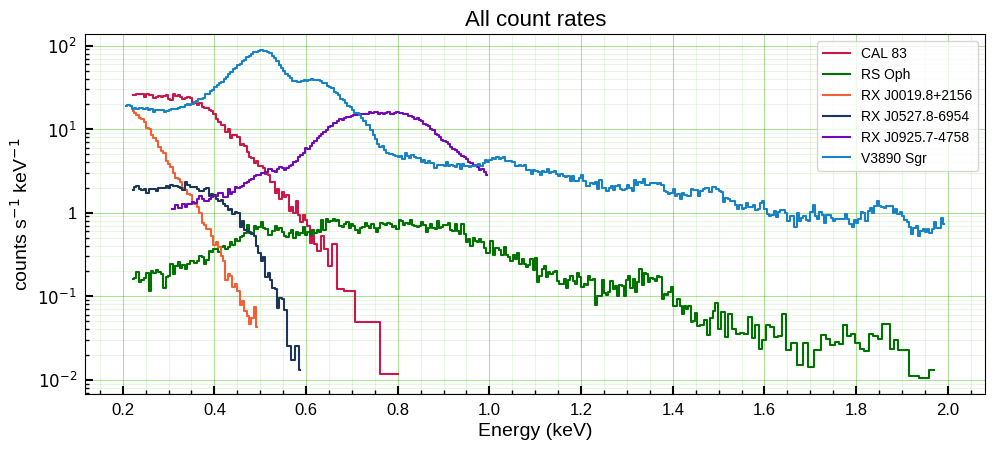
\includegraphics[width=\textwidth]{counts/all_counts}} %\hfill
				
				\subfloat[Normalized count rates of all sources \label{count-rate:rsoph}]{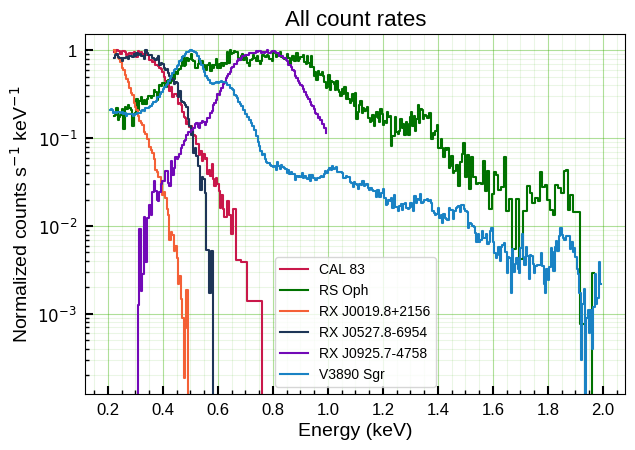
\includegraphics[width=\textwidth]{counts/all_norm-counts}} %\hfill
			\end{figure}
			
	\section{Best-fit statistics}
		The fit statistics of the best-fit model for all the sources in the dataset using continuum NLTE model is presented in table \ref{tab:sss-fit-stats}.
		\renewcommand{\arraystretch}{1.8}
		\begin{table}[!htb]
			\centering
			\caption{Fitting statistics for all sources in dataset}
			\label{tab:sss-fit-stats}
			\begin{tabular}{cccc}
				\hline
				\textbf{Source} & {$\boldsymbol{\chi^2}$/\textbf{d.o.f}} & {$\boldsymbol{\chi^2_\text{reduced}}$} & \textbf{\begin{tabular}[c]{@{}c@{}}Null hyp.\\ prob.\end{tabular}} \\ \hline
				{CAL 83} & {} & {} & {} \\
				{RS Oph} & {} & {} & {} \\
				{RX J0019.8+2156} & {$\dfrac{61.9}{51}$} & {1.21} & {$1.42\times 10^{-1}$} \\
				{RX J0527.8-6954} & {} & {} & {} \\
				{RX J0925.7-4758} & {$\dfrac{183.4}{131}$} & {1.40} & {$1.73\times 10^{-3}$} \\
				{V3890 Sgr} & {} & {} & {} \\ \hline
			\end{tabular}
		\end{table}
		\renewcommand{\arraystretch}{2.2}
		
	\section{Stellar parameters}
		The stellar parameters of all the sources in the dataset, computed using continuum NLTE model, is presented in table \ref{tab:sss-stellar-params}.
		\renewcommand{\arraystretch}{1.8}
		\begin{table}[!htb]
			\centering
			\caption{Stellar parameters of all sources from continuum NLTE model}
			\label{tab:sss-stellar-params}
			\begin{tabular}{cccc}
			\hline
			{\textbf{Source}} & {$\boldsymbol{L_*}$ \textbf{(erg s$\boldsymbol{^{-1}}$)}} & {\textbf{$\boldsymbol{T_\text{eff}}$ (kK)}} & {\textbf{$\boldsymbol{n_H}$ ($\boldsymbol{\times 10^{22}}$ cm$\boldsymbol{^{-2}}$)}} \\
			\hline
			{CAL 83} & {} & {} & {} \\
			{RS Oph} & {} & {} & {} \\
			{RX J0019.8+2156} & {$1.23_{0.39}^{2.37}\times 10^{35}$} & {$60.5_{46.5}^{70.9}$} & {$0.046_{0.014}^{0.805}$} \\
			{RX J0527.8-6954} & {} & {} & {} \\
			{RX J0925.7-4758} & {$3.05_{0.99}^{6.53}\times 10^{41}$} & {$91.6_{86.9}^{100.2}$} & {$1.175_{1.086}^{1.274}$} \\
			{V3890 Sgr} & {} & {} & {} \\
			\hline
			\end{tabular}
		\end{table}
		\renewcommand{\arraystretch}{2.2}
	
	\section{Unfolded spectra from best-fit models}
	
		\subsection{Unfolded spectrum of CAL 83}
		
		\subsection{Unfolded spectrum of RS Oph}
		
		\subsection{Unfolded spectrum of RX J0019.8+2156}
		
		\subsection{Unfolded spectrum of RX J0527.8-6954}
		
		\subsection{Unfolded spectrum of RX J0925.7-4758}
		
		\subsection{Unfolded spectrum of V3890 Sgr}
    
%    \section{Spectral Line Identification}
%    
%    \section{XMM-Newton RGS Spectral Fit}
%    The best fit model, i.e. M11, contains two different additive components that simulate optically thin plasma. One of them, i.e. \texttt{apec} uses line lists from the AtomDB database, while the other, i.e. \texttt{mekal} which is based on calculations by Mewe, Kaastra and Liedahl \cite{meka,liedahl}. The latter could indicate the presence of a hot corona. The presence of the \texttt{rauch} model component in the best fit model suggests a substantial contribution due to an NLTE stellar atmosphere. The model also consists of the \texttt{swind1} component, which simulates the presence of a stellar wind component along the line-of-sight. The presence of all the above model components vindicates our hypothesis of the inclusion of non-steady states, NLTE and stellar winds in the radiative processes in X-ray binary systems such as those of RX J0925.7-4758.
%    
%    \section{P Cygni Profiling}